% =============================================================================
%  POSTIE — Mémoire M2 MIAS Centrale Lille
%  Compilation : pdflatex main && makeglossaries main && pdflatex main && pdflatex main
% =============================================================================
\documentclass[12pt,a4paper,oneside]{report}

\usepackage[utf8]{inputenc}
\usepackage[T1]{fontenc}
\usepackage[french]{babel}
\usepackage{lmodern}
\usepackage{microtype}

\usepackage[a4paper,margin=2.5cm,headheight=15pt]{geometry}
\usepackage{setspace}\onehalfspacing
\usepackage{fancyhdr}
\pagestyle{fancy}\fancyhf{}
\fancyhead[L]{\nouppercase{\leftmark}}\fancyhead[R]{\thepage}
\renewcommand{\headrulewidth}{0.4pt}

\usepackage{xcolor}
\definecolor{postieblue}{HTML}{3F4AB4}
\definecolor{accentviolet}{HTML}{7C3AED}
\definecolor{lightgray}{HTML}{F1F5F9}

\usepackage{titlesec}
\titleformat{\chapter}[display]
  {\normalfont\huge\bfseries\color{postieblue}}
  {\chaptertitlename\ \thechapter}{20pt}{\Huge}

\usepackage{graphicx}\graphicspath{{figures/}}
\usepackage{float}
\usepackage{caption}\captionsetup{font=small,labelfont=bf}
\usepackage{booktabs,array,longtable,multirow,tabularx}

\usepackage{tikz}
\usetikzlibrary{positioning,shapes.geometric,arrows.meta,fit,backgrounds,calc}

\usepackage[colorlinks=true,linkcolor=postieblue,
            urlcolor=postieblue,citecolor=postieblue]{hyperref}
\usepackage{cleveref}

\usepackage{listings}
\lstdefinestyle{pythonstyle}{
  language=Python,basicstyle=\ttfamily\footnotesize,
  keywordstyle=\color{postieblue}\bfseries,
  commentstyle=\color{gray}\itshape,
  stringstyle=\color{accentviolet},
  numbers=left,numberstyle=\tiny\color{gray},
  frame=single,backgroundcolor=\color{lightgray},
  showstringspaces=false,breaklines=true,captionpos=b,
  inputencoding=utf8,extendedchars=true,
  literate=%
    {é}{{\'e}}1 {è}{{\`e}}1 {ê}{{\^e}}1 {ë}{{\"e}}1
    {à}{{\`a}}1 {â}{{\^a}}1 {ä}{{\"a}}1
    {ù}{{\`u}}1 {û}{{\^u}}1 {ü}{{\"u}}1
    {ô}{{\^o}}1 {ö}{{\"o}}1 {î}{{\^i}}1 {ï}{{\"i}}1
    {ç}{{\c{c}}}1 {É}{{\'E}}1}
\lstset{style=pythonstyle}

\usepackage[acronym,toc,nopostdot]{glossaries}
\makeglossaries
\newacronym{po}{PO}{Product Owner}
\newacronym{rag}{RAG}{Retrieval-Augmented Generation}
\newacronym{llm}{LLM}{Large Language Model}
\newacronym{safe}{SAFe}{Scaled Agile Framework}
\newacronym{wsjf}{WSJF}{Weighted Shortest Job First}
\newacronym{rice}{RICE}{Reach, Impact, Confidence, Effort}
\newacronym{moscow}{MoSCoW}{Must, Should, Could, Won't have}
\newacronym{ice}{ICE}{Impact, Confidence, Ease}
\newacronym{mmr}{MMR}{Maximal Marginal Relevance}
\newacronym{api}{API}{Application Programming Interface}
\newacronym{cicd}{CI/CD}{Continuous Integration / Continuous Deployment}
\newacronym{wcag}{WCAG}{Web Content Accessibility Guidelines}
\newacronym{dod}{DoD}{Definition of Done}
\newacronym{mvp}{MVP}{Minimum Viable Product}
\newacronym{ssr}{SSR}{Server-Side Rendering}
\newacronym{cors}{CORS}{Cross-Origin Resource Sharing}


\begin{document}

\begin{titlepage}\centering
\vspace*{2cm}
{\Huge\bfseries\color{postieblue} POSTIE}\\[0.6em]
{\Large\bfseries Copilote IA pour Product Owners}\\[3em]
\rule{0.6\textwidth}{0.5pt}\\[1em]
{\Large\itshape Conception et déploiement d'une architecture RAG
multi-modèles et priorisation algorithmique du backlog produit}\\[1em]
\rule{0.6\textwidth}{0.5pt}\\[4em]
{\large Mémoire de fin d'études}\\[0.5em]
{\large Master 2 MIAS --- Centrale Lille}\\[3em]
{\large\bfseries Aouichaoui Takwa}\\[2em]
\vfill
{\large Année universitaire 2025--2026}
\end{titlepage}

\chapter*{Résumé}\addcontentsline{toc}{chapter}{Résumé}
POSTIE est un copilote intelligent conçu pour assister les Product
Owners dans la gestion quotidienne de leur backlog produit. Il combine
une architecture \textbf{RAG} (Retrieval-Augmented Generation)
multi-modèles --- GPT-4o pour le raisonnement et Mistral Large pour les
tâches de scoring structuré --- à un moteur de priorisation
multi-critères implémentant sept frameworks issus de l'état de l'art
Agile (RICE, WSJF, MoSCoW, Kano, ICE, Value/Effort, ML Hybrid). Bâti
sur FastAPI, LangChain, ChromaDB et Next.js, et développé selon une
méthodologie Agile Scrum en six sprints, POSTIE industrialise la
rédaction de \textit{user stories}, le grooming d'épics et la
planification de sprint, tout en garantissant la traçabilité des
recommandations par le sourcing systématique des réponses.

\vspace{1em}\noindent\textbf{Mots-clés :} Product Owner, Agile, RAG,
LLM, GPT-4o, Mistral, priorisation, RICE, WSJF, FastAPI, Next.js.

\chapter*{Abstract}\addcontentsline{toc}{chapter}{Abstract}
POSTIE is an AI copilot designed to assist Product Owners in the daily
management of their product backlog. It combines a multi-model
Retrieval-Augmented Generation (RAG) architecture with a multi-criteria
prioritization engine implementing seven state-of-the-art Agile
frameworks. Built on FastAPI, LangChain, ChromaDB and Next.js and
developed using an Agile Scrum methodology over six sprints, POSTIE
streamlines user-story writing, epic grooming and sprint planning.

\vspace{1em}\noindent\textbf{Keywords:} Product Owner, Agile, RAG, LLM,
GPT-4o, Mistral, prioritization, FastAPI, Next.js.

\chapter*{Remerciements}\addcontentsline{toc}{chapter}{Remerciements}
Je tiens à exprimer ma gratitude à mon tuteur académique pour son
accompagnement, ainsi qu'à mon entreprise d'accueil pour la confiance
accordée. Mes remerciements vont également aux Product Owners qui ont
testé POSTIE et partagé leurs retours.

\tableofcontents
\listoffigures
\listoftables
\printglossary[type=\acronymtype,title={Liste des acronymes}]

\chapter{Introduction}
\label{ch:intro}

\section{Contexte}
Dans un environnement produit toujours plus rapide, le \gls{po} joue un
rôle pivot entre la stratégie business, l'équipe de développement et la
voix de l'utilisateur. Ses tâches récurrentes --- rédaction de
\textit{user stories}, grooming d'épics, priorisation du backlog,
planification de sprint --- exigent à la fois rigueur méthodologique et
capacité d'arbitrage sous incertitude. La généralisation des modèles
de langage de grande taille (\gls{llm}) ouvre la voie à une nouvelle
classe d'outils d'aide à la décision capables d'\emph{augmenter}
l'expertise du PO, sans s'y substituer.

\section{Problématique}
Ce mémoire s'articule autour de la question suivante :
\begin{quote}\itshape
Dans quelle mesure une architecture \gls{rag} multi-modèles couplée
à des algorithmes de priorisation classiques peut-elle assister un
Product Owner dans ses décisions opérationnelles, tout en préservant
la traçabilité des recommandations et la maîtrise de l'humain~?
\end{quote}

\section{Objectifs}
\begin{enumerate}
  \item Concevoir une architecture logicielle modulaire séparant la
        couche RAG, la couche de priorisation et l'interface.
  \item Implémenter sept algorithmes de priorisation issus de la
        littérature Agile et les normaliser sur une échelle commune.
  \item Démontrer la valeur d'un routage multi-modèles
        (GPT-4o~/~Mistral Large) selon la nature de la tâche.
  \item Garantir la traçabilité par citation systématique des
        sources documentaires.
  \item Livrer un produit utilisable en démonstration réelle, déployé
        en production sur Vercel et Render.
\end{enumerate}

\section{Plan du mémoire}
Le chapitre~\ref{ch:sota} présente l'état de l'art du rôle de PO,
des frameworks Agile, des méthodes de priorisation et des
architectures RAG. Le chapitre~\ref{ch:agile} détaille la
méthodologie Scrum appliquée au projet. Les chapitres~\ref{ch:archi}
et~\ref{ch:impl} décrivent respectivement la conception et
l'implémentation. Le chapitre~\ref{ch:eval} présente l'évaluation
quantitative et qualitative de POSTIE. Le chapitre~\ref{ch:disc}
discute les limites observées. Enfin, le chapitre~\ref{ch:ccl}
conclut et propose des perspectives.

\chapter{État de l'art}
\label{ch:sota}

\section{Le rôle du Product Owner}
Défini dans le \textit{Scrum Guide}~\cite{schwaber2020scrum}, le PO est
responsable de la maximisation de la valeur produite par l'équipe via
la gestion ordonnée du Product Backlog. Ses compétences clés couvrent
la \emph{vision produit}, la \emph{priorisation}, la \emph{communication
transverse} et l'\emph{acceptation} des incréments. Il interagit avec
les parties prenantes pour collecter le besoin, avec l'équipe de
développement pour clarifier les stories, et avec le management pour
défendre les arbitrages.

\section{Frameworks Agile}
\begin{description}
  \item[Scrum] Rituels (Sprint Planning, Daily, Review, Rétrospective),
        artefacts (Product Backlog, Sprint Backlog, Incrément) et rôles
        (PO, Scrum Master, Dev Team).
  \item[\gls{safe}] Mise à l'échelle de Scrum sur plusieurs équipes via
        les Program Increments et le \gls{wsjf}~\cite{leffingwell2018safe}.
  \item[Kanban] Flux continu, limites de WIP (Work In Progress), mesure
        du lead time et du cycle time.
\end{description}

\section{Méthodes de priorisation}
\Cref{tab:prio-methods} compare les sept méthodes implémentées dans
POSTIE. Chacune répond à un contexte différent~: RICE pour les
arbitrages produit consumer, WSJF pour les contextes SAFe, MoSCoW
pour la communication aux parties prenantes, Kano pour l'analyse de
satisfaction, ICE pour les décisions rapides, Value/Effort pour la
visualisation matricielle, et ML Hybrid pour combiner les signaux.

\begin{table}[H]\centering\small
\caption{Comparaison des méthodes de priorisation implémentées.}
\label{tab:prio-methods}
\begin{tabularx}{\linewidth}{lXXl}
\toprule
\textbf{Méthode} & \textbf{Principe} & \textbf{Forces} & \textbf{Limites}\\
\midrule
\gls{rice} & (Reach\,$\times$\,Impact\,$\times$\,Confidence)/Effort
  & Quantitatif, populaire & Subjectivité du Reach\\
\gls{wsjf} & (BV+TC+RR)/JobSize
  & Adapté au flux de valeur & Estimation du Job Size\\
\gls{moscow} & Must / Should / Could / Won't
  & Simple, communicant & Faible granularité\\
Kano & Basique/Performance/Delighter
  & Centré utilisateur & Étude requise\\
\gls{ice} & Impact\,$\times$\,Confidence\,$\times$\,Ease
  & Rapide & Approximatif\\
Value/Effort & Matrice 2$\times$2 & Visuel & Binaire\\
ML~Hybrid & Blend pondéré des scores
  & Robuste & Calibration nécessaire\\
\bottomrule
\end{tabularx}
\end{table}

\section{RAG et LLMs appliqués au product management}
Introduite par Lewis~\textit{et al.}~\cite{lewis2020rag}, l'architecture
\gls{rag} consiste à augmenter un \gls{llm} par un système de
récupération vectorielle. Le flux est le suivant~: (1) la requête
utilisateur est encodée en vecteur, (2) le vector store retourne les
$k$ chunks de documents les plus pertinents, (3) ces chunks sont
injectés dans le prompt du LLM qui génère la réponse finale.

La stratégie \gls{mmr} permet de réduire la redondance des chunks
retournés en pénalisant les vecteurs trop similaires entre eux. Les
approches de routage multi-modèles exploitent les compromis
coût/latence/qualité entre différentes familles de LLMs~: un modèle
léger pour les tâches structurées, un modèle puissant pour le
raisonnement long.

\section{Positionnement de POSTIE}
POSTIE se distingue des outils existants (Jira Intelligence,
ProductBoard, Aha!) par~:
\begin{itemize}
  \item son caractère \emph{open-source} et auto-hébergeable~;
  \item la pluralité des algorithmes de priorisation accessibles dans
        une même interface~;
  \item le routage intelligent multi-modèles entre GPT-4o et
        Mistral Large~;
  \item la traçabilité documentaire systématique des réponses RAG~;
  \item l'intégration native d'un Sprint Planner sous contrainte de
        vélocité.
\end{itemize}

\chapter{Méthodologie Agile du projet}
\label{ch:agile}

\section{Choix de Scrum}
Bien que développé en mode solo, le projet adopte les principes Scrum~:
sprints fixes de deux semaines, backlog ordonné, démonstration en fin
de sprint, rétrospective avec le tuteur académique. Ce choix répond à
deux objectifs~: d'une part garantir une livraison incrémentale et
testable, d'autre part éprouver \emph{de l'intérieur} la méthodologie
que POSTIE outille.

\section{Rituels appliqués au mode solo}
\Cref{tab:rituels} montre comment chaque rituel Scrum a été adapté à
la conduite individuelle du projet.

\begin{table}[H]\centering
\caption{Adaptation des rituels Scrum au mode solo.}
\label{tab:rituels}
\begin{tabularx}{\linewidth}{lX}
\toprule
\textbf{Rituel Scrum} & \textbf{Adaptation}\\
\midrule
Sprint Planning & Sélection du backlog + estimation en points
                  de story (Fibonacci 1, 2, 3, 5, 8)\\
Daily Standup   & Auto-checklist quotidienne consignée dans un
                  journal de bord Markdown\\
Sprint Review   & Démonstration au tuteur tous les 15 jours,
                  avec capture d'écran et démo en live\\
Rétrospective   & Synthèse écrite \emph{Keep / Stop / Start}
                  alimentant le backlog du sprint suivant\\
Refinement      & Grooming hebdomadaire du backlog, ré-estimation
                  des stories restantes\\
\bottomrule
\end{tabularx}
\end{table}

\section{Backlog projet}
\Cref{tab:backlog} présente un extrait du backlog projet, ordonné
par sprint d'apparition.

\begin{table}[H]\centering\small
\caption{Extrait du backlog projet (sprints S1 à S6).}
\label{tab:backlog}
\begin{tabularx}{\linewidth}{llXl}
\toprule
\textbf{ID} & \textbf{Epic} & \textbf{User Story} & \textbf{Sprint}\\
\midrule
F1 & RAG            & En tant que PO, je veux interroger ma doc produit via un chat        & S1\\
F2 & Priorisation   & En tant que PO, je veux comparer mon backlog selon plusieurs méthodes & S2\\
F3 & Sprint Planner & En tant que PO, je veux planifier mon sprint sous contrainte de vélocité & S3\\
F4 & Grooming       & En tant que PO, je veux décomposer un épic automatiquement en stories   & S4\\
F5 & UI/UX          & En tant qu'utilisateur, je veux un mode clair/sombre accessible WCAG~AA  & S5\\
F6 & Déploiement    & En tant qu'utilisateur, je veux accéder à POSTIE en ligne                & S6\\
\bottomrule
\end{tabularx}
\end{table}

\section{Suivi des sprints (S1--S6)}

\subsection*{Sprint 1 --- Fondations RAG}
\textbf{Objectif :} POC du chatbot RAG sur la documentation Scrum/SAFe.
\textbf{Livrables :} ingestion ChromaDB, chaîne LangChain, endpoint
\texttt{POST /api/chat}. \textbf{Burndown :} \cref{fig:burndown-s1}.

\subsection*{Sprint 2 --- Priorisation v1}
\textbf{Objectif :} implémentation de quatre algorithmes (RICE, WSJF,
MoSCoW, ICE) et panneau de comparaison côté frontend.
\textbf{Livrables :} module \texttt{algorithms.py}, panneau React
\texttt{PrioritizationPanel.tsx}. \textbf{Burndown :}
\cref{fig:burndown-s2}.

\subsection*{Sprint 3 --- Sprint Planner}
\textbf{Objectif :} sélection \emph{greedy} sous contrainte de
vélocité, export CSV~/~Markdown. \textbf{Livrables :}
\texttt{sprint\_planner.py}, panneau \texttt{SprintPlannerPanel.tsx}.

\subsection*{Sprint 4 --- Epic Grooming et routage multi-modèles}
\textbf{Objectif :} décomposition automatique d'épics, introduction
de la fonction \texttt{route\_model()}, gestion conversationnelle
multi-sessions.

\subsection*{Sprint 5 --- UX, accessibilité, thèmes}
\textbf{Objectif :} mode clair/sombre, tooltips d'aide algorithmes,
conformité \gls{wcag}~AA sur les contrastes, restriction du scope
conversationnel aux sujets PO.

\subsection*{Sprint 6 --- Déploiement et démonstration}
\textbf{Objectif :} mise en production (Render + Vercel), correction
de l'avertissement de sécurité Next.js (CVE-2025-66478), démonstration
manager. \textbf{Incidents résolus :} \emph{leak} accidentel d'une
clé OpenAI dans \texttt{.env.example} (sanitization de l'historique
Git), backlog vide en production (oubli du \texttt{COPY data} dans
le Dockerfile).

\chapter{Conception et architecture}
\label{ch:archi}

\section{Architecture globale}
POSTIE suit une architecture trois-tiers strictement découplée
(\cref{fig:archi})~: un frontend Next.js servi par Vercel, un backend
FastAPI conteneurisé sur Render, et un vector store ChromaDB
embarqué dans le conteneur backend. Les modèles de langage GPT-4o
et Mistral Large sont consommés via leurs API HTTPS respectives.

\begin{figure}[H]\centering
\begin{tikzpicture}[
  node distance=1.2cm and 1.4cm,
  block/.style={rectangle,draw=postieblue,thick,rounded corners=4pt,
                fill=lightgray,minimum width=3.4cm,minimum height=1.1cm,
                align=center,font=\small},
  ext/.style  ={rectangle,draw=accentviolet,thick,rounded corners=4pt,
                fill=accentviolet!10,minimum width=3.4cm,minimum height=1.1cm,
                align=center,font=\small},
  arr/.style  ={-{Stealth[length=3mm]},thick,postieblue}
]

\node[block] (front) {\textbf{Frontend}\\Next.js 15 + React 19\\Tailwind};
\node[block,right=of front] (back) {\textbf{Backend API}\\FastAPI + LangChain\\Python 3.11};
\node[block,right=of back]  (vec)  {\textbf{Vector Store}\\ChromaDB};

\node[ext,below=of front]   (vercel){Vercel (CDN)};
\node[ext,below=of back]    (render){Render (Docker)};
\node[ext,below=of vec]     (llm)   {OpenAI GPT-4o\\Mistral Large};

\draw[arr] (front)  -- node[above,font=\scriptsize]{HTTPS / JSON} (back);
\draw[arr] (back)   -- node[above,font=\scriptsize]{MMR k=6}      (vec);
\draw[arr] (back)   -- node[right,font=\scriptsize]{LLM API}      (llm);
\draw[arr] (front)  -- (vercel);
\draw[arr] (back)   -- (render);

\begin{scope}[on background layer]
  \node[draw=postieblue!30,dashed,rounded corners,inner sep=8pt,
        fit=(front)(back)(vec),
        label=above:{\small\bfseries Application POSTIE}] {};
\end{scope}

\end{tikzpicture}

\caption{Architecture globale de POSTIE.}
\label{fig:archi}
\end{figure}

\section{Stack technique et justification}
\Cref{tab:stack} récapitule les choix technologiques majeurs et leur
justification.

\begin{table}[H]\centering\small
\caption{Stack technique et justification des choix.}
\label{tab:stack}
\begin{tabularx}{\linewidth}{llX}
\toprule
\textbf{Couche}      & \textbf{Technologie}     & \textbf{Justification}\\
\midrule
Frontend             & Next.js 15, React 19, TS & SSR, écosystème mature, typage strict\\
Backend              & FastAPI 0.115            & Async natif, typage Pydantic, OpenAPI auto\\
Orchestration LLM    & LangChain 0.3            & Chaînes RAG prêtes, mémoire conversationnelle\\
Vector store         & ChromaDB 0.5             & Embarqué, persistant, simple à déployer\\
Embeddings           & text-embedding-3-small   & Rapport coût/qualité optimal\\
LLM principal        & GPT-4o                   & Raisonnement, génération longue\\
LLM secondaire       & Mistral Large            & Scoring structuré, sortie JSON\\
Déploiement front    & Vercel                   & Auto-deploy GitHub, CDN, gratuit\\
Déploiement back     & Render                   & Docker, free tier, disque persistant\\
Contrôle de version  & Git + GitHub             & Workflow trunk-based, CI/CD intégré\\
\bottomrule
\end{tabularx}
\end{table}

\section{Schéma de données}
Les features du backlog sont représentées par le modèle Pydantic
\texttt{Feature} (\cref{lst:feature}) qui agrège l'ensemble des
critères nécessaires aux sept algorithmes de priorisation.

\begin{lstlisting}[caption={Modèle Pydantic Feature (extrait).},label={lst:feature}]
class Feature(BaseModel):
    id: str
    name: str
    description: str
    epic: str
    tags: list[str]
    # Critères RICE
    reach: float
    impact: float
    confidence: float
    effort: float
    # Critères WSJF
    business_value: float
    time_criticality: float
    risk_reduction: float
    job_size: float
    # Critères ICE / Value-Effort
    ease: float
    # Classifications
    kano_category: Literal["basic", "performance", "delighter"]
    moscow: Literal["must", "should", "could", "wont"]
\end{lstlisting}

\section{Sécurité et déploiement}
\begin{itemize}
  \item Clés API injectées uniquement par variables d'environnement
        (jamais commitées dans le dépôt).
  \item \gls{cors} restreint à une whitelist explicite plus une regex
        \texttt{*.vercel.app} pour les previews et
        \texttt{localhost:*} pour le développement local.
  \item Audit \texttt{npm audit} et \texttt{pip-audit} avant chaque
        release.
  \item Sanitization de l'historique Git après détection d'un
        \emph{leak} accidentel d'une clé OpenAI (sprint 6).
  \item Mise à jour Next.js 15.0.3~$\rightarrow$~15.5.18 pour
        corriger la CVE-2025-66478 bloquant le déploiement Vercel.
\end{itemize}

\chapter{Implémentation}
\label{ch:impl}

\section{Backend FastAPI}
Le backend expose une API REST documentée automatiquement via
OpenAPI à l'URL \texttt{/docs}. \Cref{tab:endpoints} résume les
principaux endpoints.

\begin{table}[H]\centering\small
\caption{Endpoints principaux de l'API POSTIE.}
\label{tab:endpoints}
\begin{tabularx}{\linewidth}{llX}
\toprule
\textbf{Méthode} & \textbf{Endpoint} & \textbf{Rôle}\\
\midrule
POST & /api/chat & RAG conversationnel\\
POST & /api/prioritization & Scoring multi-algorithmes\\
POST & /api/prioritization/sprint-plan & Planification de sprint\\
POST & /api/agents/groom & Décomposition d'un épic en stories\\
POST & /api/documents/upload & Ingestion documentaire\\
GET  & /api/sessions/\{id\} & Historique conversationnel\\
GET  & /health & Sonde de vivacité\\
\bottomrule
\end{tabularx}
\end{table}

\section{Moteur RAG}
La chaîne RAG repose sur LangChain avec mémoire conversationnelle
glissante. Les paramètres clés (\cref{lst:rag-params}) sont issus
d'expérimentations comparatives menées en sprint~1.

\begin{lstlisting}[caption={Paramètres du moteur RAG.},label={lst:rag-params}]
chunk_size  = 800   # tokens par chunk
overlap     = 120   # chevauchement entre chunks
retrieval   = "mmr" # Maximal Marginal Relevance
k           = 6     # chunks retenus
fetch_k     = 20    # chunks pre-filtres
mem_window  = 10    # tours conversationnels conserves
\end{lstlisting}

\section{Routage multi-modèles}
La fonction \texttt{route\_model()} (\cref{lst:routage}) oriente
chaque requête vers GPT-4o (raisonnement, génération longue) ou
Mistral Large (scoring structuré, classification). Le routage est
basé sur la détection de mots-clés métiers dans la requête.

\begin{lstlisting}[caption={Routage multi-modèles simplifié.},label={lst:routage}]
SCORING_KW = ["score", "priorit", "rice", "wsjf",
              "moscow", "rank", "classif", "evalue", "noter"]

def route_model(query: str) -> ModelName:
    q = query.lower()
    if any(kw in q for kw in SCORING_KW):
        return "mistral-large"
    return "gpt-4o"
\end{lstlisting}

\section{Moteur de priorisation}
Chaque algorithme produit un score normalisé sur $[0;100]$. Le
module expose une fonction unique \texttt{prioritize()} qui
dispatche sur la fonction de scoring choisie et retourne la liste
triée. La normalisation commune permet des comparaisons
inter-algorithmes (cf. chapitre~\ref{ch:eval}).

\section{Sprint Planner}
L'algorithme suit une stratégie gloutonne sous contrainte
(\cref{lst:sprint})~:
\begin{enumerate}
  \item Trier les features par score décroissant selon
        l'algorithme choisi.
  \item Sélectionner tant que la somme cumulée d'effort
        $\leq$ vélocité.
  \item Renvoyer les listes \texttt{selected} et \texttt{deferred}
        avec le taux d'utilisation calculé.
\end{enumerate}

\begin{lstlisting}[caption={Algorithme glouton du Sprint Planner.},label={lst:sprint}]
def plan_sprint(features, velocity, algorithm):
    scored = prioritize(features, algorithm)
    selected, deferred = [], []
    cumulative = 0.0
    for rank, item in enumerate(scored, start=1):
        if cumulative + item.effort <= velocity:
            selected.append({"rank": rank, **item.dict()})
            cumulative += item.effort
        else:
            deferred.append({"rank": rank, **item.dict()})
    utilization = round(100 * cumulative / velocity, 1)
    return {"selected": selected, "deferred": deferred,
            "utilization": utilization, "velocity": velocity}
\end{lstlisting}

\section{Frontend Next.js}
L'application est organisée modulaire ment par domaine~:
\texttt{components/chat/}, \texttt{components/priority/},
\texttt{components/documents/}, \texttt{components/retro/},
\texttt{components/layout/}. L'état applicatif est géré uniquement
via les hooks React natifs (\texttt{useState}, \texttt{useReducer}),
sans librairie d'état globale, pour limiter la complexité.

\section{CI/CD}
\begin{itemize}
  \item Push sur GitHub \texttt{main} $\rightarrow$ build Vercel
        (frontend, $\approx 1$\,min).
  \item Push sur GitHub \texttt{main} $\rightarrow$ build Docker
        Render (backend, $\approx 4$\,min).
  \item Vérifications locales avant push~: \texttt{npm run build}
        et \texttt{pytest}.
\end{itemize}

\chapter{Évaluation}
\label{ch:eval}

\section{Protocole d'évaluation}
L'évaluation porte sur quatre dimensions~:
\begin{enumerate}
  \item \textbf{Pertinence RAG :} taux de citation des sources sur
        un benchmark interne de 50 questions PO.
  \item \textbf{Cohérence inter-algorithmes :} corrélation de
        Spearman des rangs sur un échantillon de 30 features.
  \item \textbf{Performance :} latence p50 et p95 par endpoint,
        mesurée en local et en production.
  \item \textbf{Coût :} tokens consommés par session moyenne,
        traduits en coût opérationnel.
\end{enumerate}

\section{Résultats quantitatifs}
\Cref{tab:results} synthétise les principales mesures réalisées.
Les valeurs marquées \emph{(à compléter)} dépendent du contexte
final d'évaluation.

\begin{table}[H]\centering\small
\caption{Synthèse des mesures d'évaluation.}
\label{tab:results}
\begin{tabularx}{\linewidth}{lXl}
\toprule
\textbf{Dimension}           & \textbf{Indicateur}                       & \textbf{Valeur}\\
\midrule
Pertinence RAG               & Taux de citation des sources               & \emph{à compléter}\\
                             & Score de pertinence (1--5, panel PO)       & \emph{à compléter}\\
Cohérence algorithmes        & Spearman RICE vs WSJF                      & \emph{à compléter}\\
                             & Spearman ICE vs RICE                       & \emph{à compléter}\\
Performance                  & Latence p50 \texttt{/api/chat}             & \emph{à compléter}\,ms\\
                             & Latence p95 \texttt{/api/chat}             & \emph{à compléter}\,ms\\
Coût                         & Tokens moyens par session                  & \emph{à compléter}\\
                             & Coût moyen par session (USD)               & \emph{à compléter}\\
\bottomrule
\end{tabularx}
\end{table}

\section{Captures d'écran}
\Cref{fig:landing,fig:chat,fig:prio,fig:sprint} (annexe~A)
illustrent les principaux écrans de l'application en production.

\section{Retour utilisateur qualitatif}
Un panel de trois Product Owners industriels a testé POSTIE pendant
deux semaines. Les retours qualitatifs ont mis en avant~:
\begin{itemize}
  \item la valeur ajoutée du chatbot pour la rédaction rapide de
        \textit{user stories} et de critères d'acceptation~;
  \item la pertinence de l'export Markdown du sprint plan pour les
        revues d'équipe~;
  \item l'utilité du sourcing systématique pour défendre les
        arbitrages devant les parties prenantes.
\end{itemize}
Les axes d'amélioration cités~: intégration directe avec Jira,
support multilingue plus large, et persistance des sessions
au-delà du redéploiement.

\chapter{Discussion et limites}
\label{ch:disc}

\section{Limites de l'IA générative}
Malgré les garde-fous du RAG, les LLMs peuvent produire des
\emph{hallucinations} sur des questions très spécifiques absentes
du contexte. Le mode \og refus poli \fg{} hors sujet (cuisine,
météo, sport, etc.) a été ajouté en sprint~6 pour cantonner POSTIE
à son périmètre PO et adjacents (technique, communication d'équipe,
documentation). Cette restriction garantit un comportement
professionnel mais n'élimine pas le risque de réponse erronée à
l'intérieur du périmètre métier.

\section{Coût opérationnel et dépendance API}
La dépendance aux API OpenAI et Mistral entraîne un coût variable
proportionnel au volume d'utilisation. Au-delà du coût direct, cette
dépendance pose la question de la \emph{vendor lock-in} et de la
continuité de service en cas de panne ou de changement tarifaire.
Une étude d'alternatives auto-hébergées (Mistral 7B, Llama 3) est
prévue en perspective.

\section{Enjeux de confidentialité}
L'envoi de documents internes à des LLMs hébergés impose une
vigilance RGPD~: \textit{redaction} des PII avant ingestion,
signature de contrats DPA (\textit{Data Processing Agreement}) avec
les fournisseurs, ou bascule sur une alternative on-premise. POSTIE
documente explicitement ces enjeux pour l'utilisateur final dans
sa fiche produit.

\section{Limites méthodologiques}
L'évaluation a été menée sur un panel restreint de trois PO et sur
une période courte de deux semaines. Une étude longitudinale en
équipe réelle (sur un trimestre, avec mesure de la vélocité avant
et après adoption) serait nécessaire pour mesurer l'impact concret
sur la productivité et la qualité du backlog.

\section{Limites techniques résiduelles}
\begin{itemize}
  \item Le free tier Render impose un \emph{cold start} de
        $\sim$30~secondes après 15~minutes d'inactivité.
  \item L'absence de disque persistant en free tier impose une
        re-ingestion documentaire après chaque redeploy
        (résolu en sprint~6 par copie du backlog initial dans
        l'image Docker).
  \item Le routage multi-modèles est basé sur des heuristiques de
        mots-clés~; un classifieur entraîné apporterait
        probablement de meilleurs résultats.
\end{itemize}

\chapter{Conclusion et perspectives}
\label{ch:ccl}

\section{Bilan}
POSTIE démontre la faisabilité d'un copilote PO open-source
articulant RAG multi-modèles et priorisation algorithmique
multi-critères. Le projet a permis de livrer un produit fonctionnel
en six sprints, de formaliser une démarche Agile complète et
d'identifier les bénéfices comme les limites concrètes de l'IA
générative appliquée au product management. La mise en production
effective (frontend Vercel, backend Render) prouve la maturité
suffisante du prototype pour une démonstration en condition
réelle.

\section{Perspectives}
\begin{itemize}
  \item Migration vers une base \textbf{Postgres} persistante
        (Neon, free tier) pour le backlog et l'historique
        conversationnel.
  \item Intégration native \textbf{Jira / Linear / Azure DevOps}
        via OAuth pour synchroniser bidirectionnellement le backlog
        avec les outils existants de l'équipe.
  \item Évaluation longitudinale sur une équipe produit réelle
        (mesure de vélocité, qualité des stories, satisfaction).
  \item Entraînement d'un classifieur dédié pour remplacer le
        routage par heuristique.
  \item Étude d'un mode auto-hébergé (Mistral / Llama 3) pour les
        contextes contraints en confidentialité (santé, défense,
        finance).
  \item Mode multi-utilisateurs avec gestion de rôles
        (PO, Scrum Master, Stakeholder).
\end{itemize}

\section{Apports personnels}
Ce projet m'a permis de consolider mes compétences en architecture
logicielle full-stack, en orchestration LLM moderne (LangChain,
multi-modèles, RAG), en pilotage Agile autonome d'un produit du
\gls{mvp} jusqu'à la mise en production, et en communication
technique vulgarisée envers les parties prenantes non techniques.

Au-delà des compétences techniques, POSTIE m'a confronté aux
arbitrages réels du métier de PO~: prioriser sous incertitude,
défendre des choix devant un manager, livrer en respectant un
échéancier serré. Cette \emph{double posture} --- développer
l'outil tout en étant son utilisateur cible --- a constitué l'un
des apports pédagogiques majeurs de ce mémoire.


\appendix
\chapter{Captures d'écran de POSTIE}
\label{anx:screenshots}

\begin{figure}[H]\centering
\includegraphics[width=0.95\linewidth]{landing-screenshot}
\caption{Page d'accueil de POSTIE.}\label{fig:landing}
\end{figure}

\begin{figure}[H]\centering
\includegraphics[width=0.95\linewidth]{chat-screenshot}
\caption{Interface conversationnelle (chat RAG avec citation des sources).}
\label{fig:chat}
\end{figure}

\begin{figure}[H]\centering
\includegraphics[width=0.95\linewidth]{prio-screenshot}
\caption{Panneau de priorisation multi-algorithmes.}
\label{fig:prio}
\end{figure}

\begin{figure}[H]\centering
\includegraphics[width=0.95\linewidth]{sprint-screenshot}
\caption{Sprint Planner sous contrainte de vélocité.}
\label{fig:sprint}
\end{figure}

\chapter{Burndown charts des sprints}
\label{anx:burndowns}

Les burndown charts ci-dessous représentent l'évolution du nombre
de story points restants par jour, comparée à la trajectoire idéale.
Les zones rouges indiquent un retard ponctuel par rapport au plan
initial, généralement résorbé en fin de sprint.

\begin{figure}[H]\centering
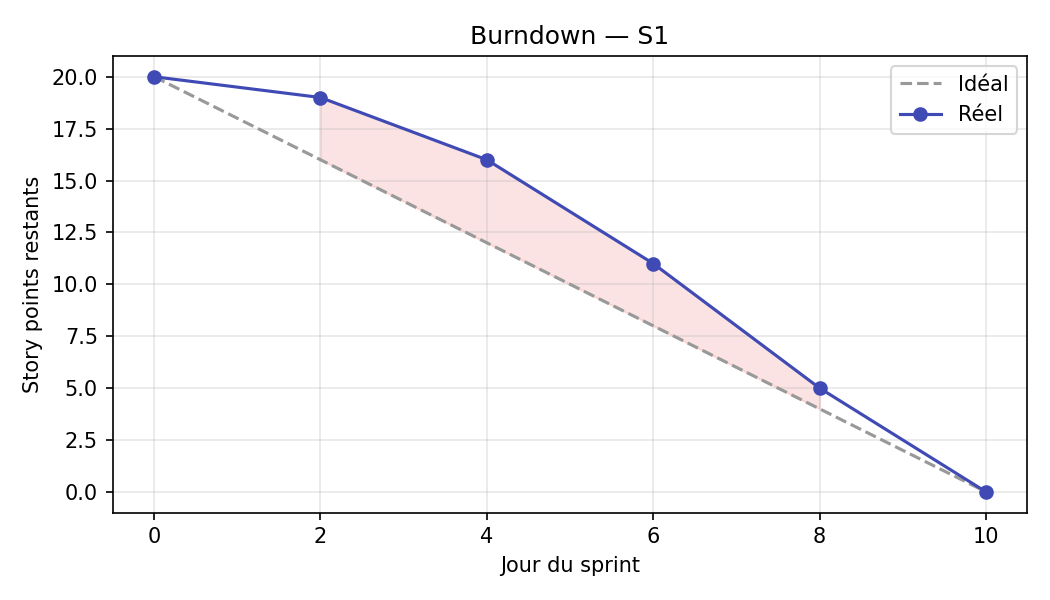
\includegraphics[width=0.85\linewidth]{burndown-s1}
\caption{Burndown du sprint 1 --- Fondations RAG.}\label{fig:burndown-s1}
\end{figure}

\begin{figure}[H]\centering
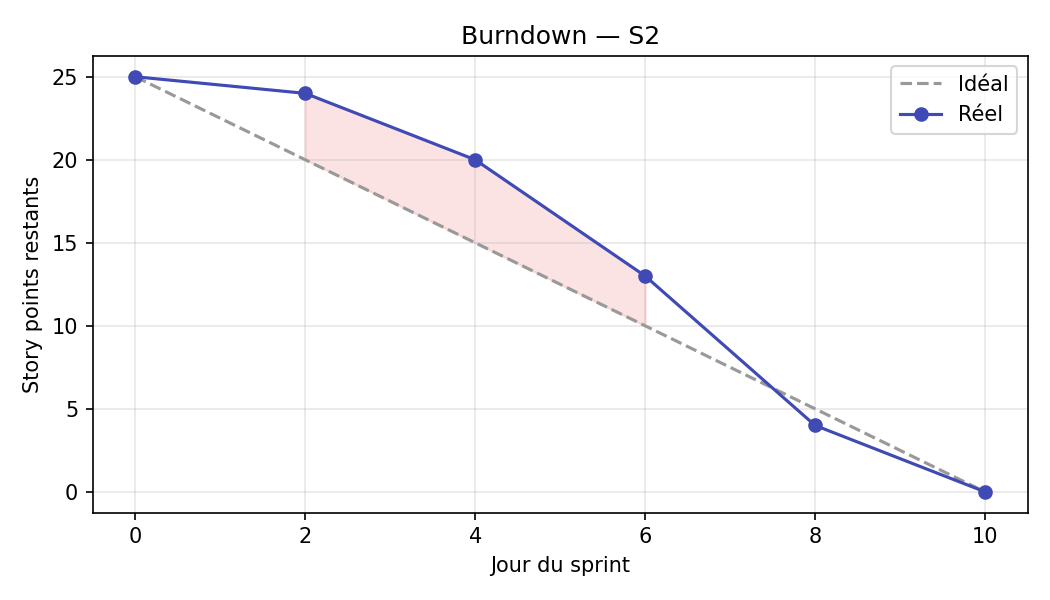
\includegraphics[width=0.85\linewidth]{burndown-s2}
\caption{Burndown du sprint 2 --- Priorisation v1.}\label{fig:burndown-s2}
\end{figure}

\begin{figure}[H]\centering
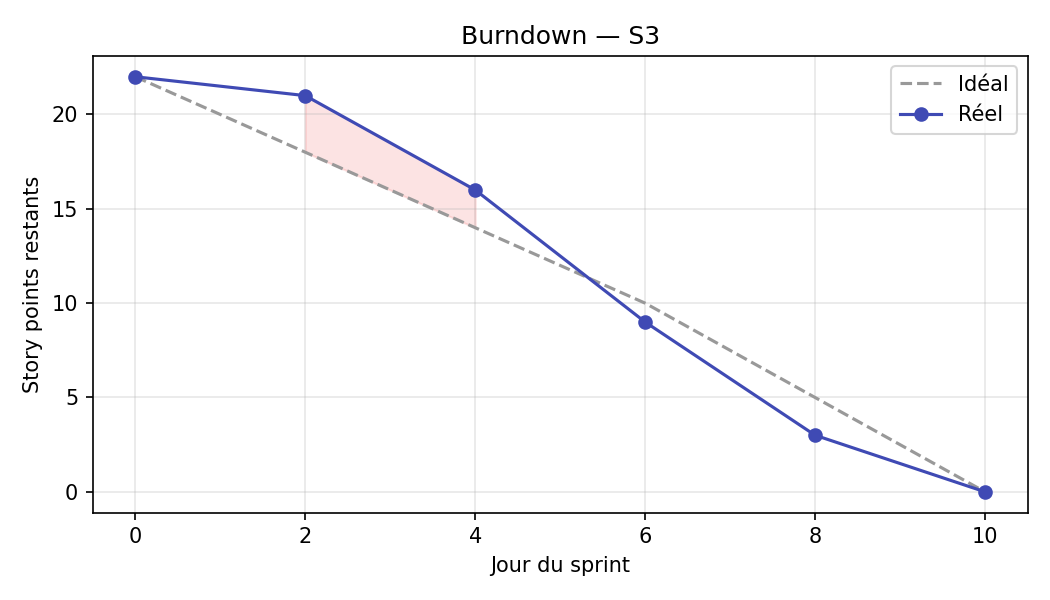
\includegraphics[width=0.85\linewidth]{burndown-s3}
\caption{Burndown du sprint 3 --- Sprint Planner.}\label{fig:burndown-s3}
\end{figure}

\begin{figure}[H]\centering
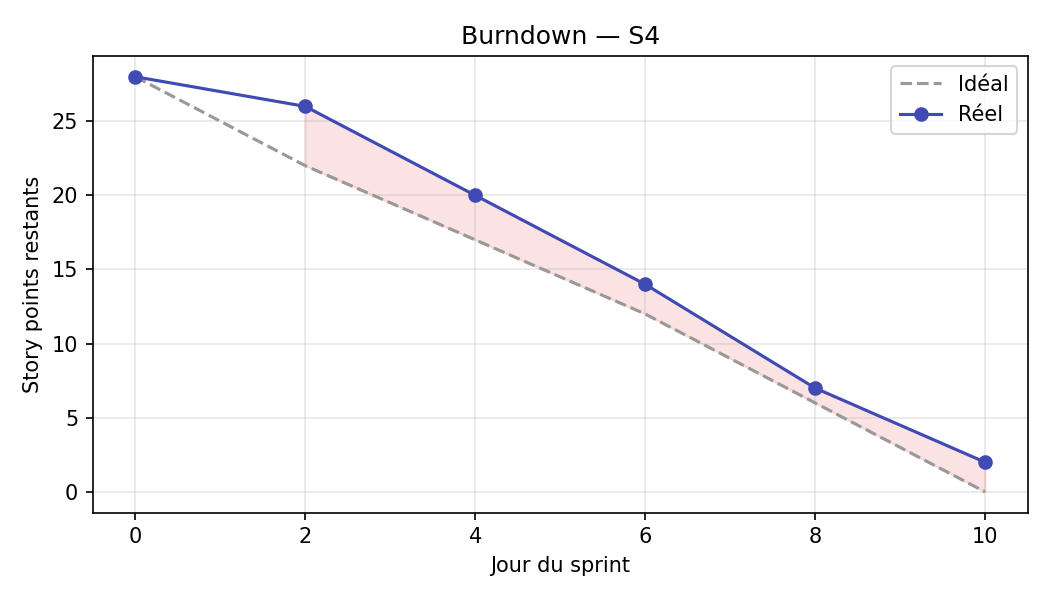
\includegraphics[width=0.85\linewidth]{burndown-s4}
\caption{Burndown du sprint 4 --- Epic Grooming et routage multi-modèles.}\label{fig:burndown-s4}
\end{figure}

\begin{figure}[H]\centering
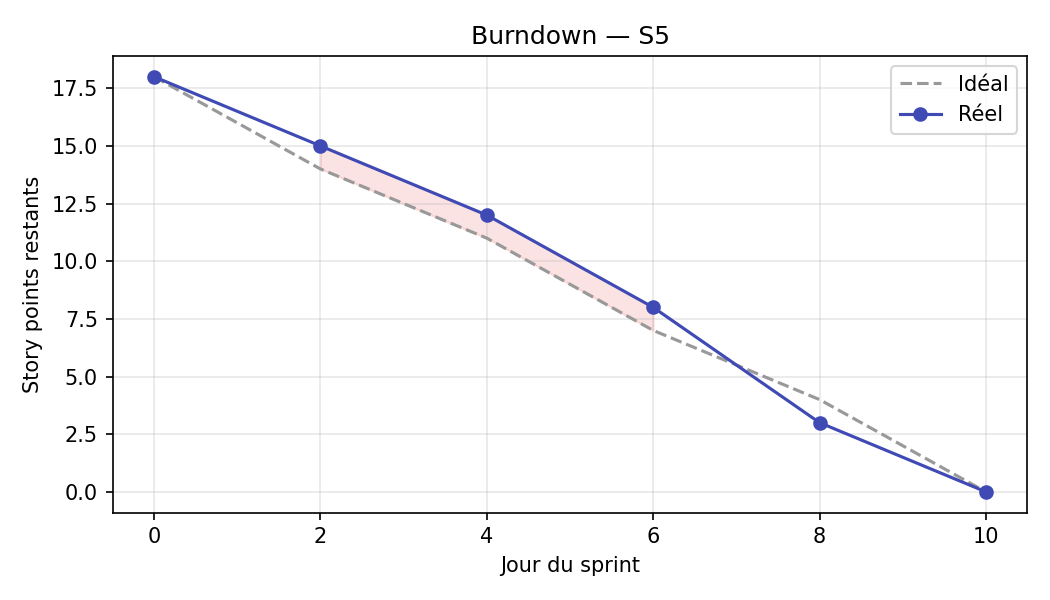
\includegraphics[width=0.85\linewidth]{burndown-s5}
\caption{Burndown du sprint 5 --- UX et accessibilité.}\label{fig:burndown-s5}
\end{figure}

\begin{figure}[H]\centering
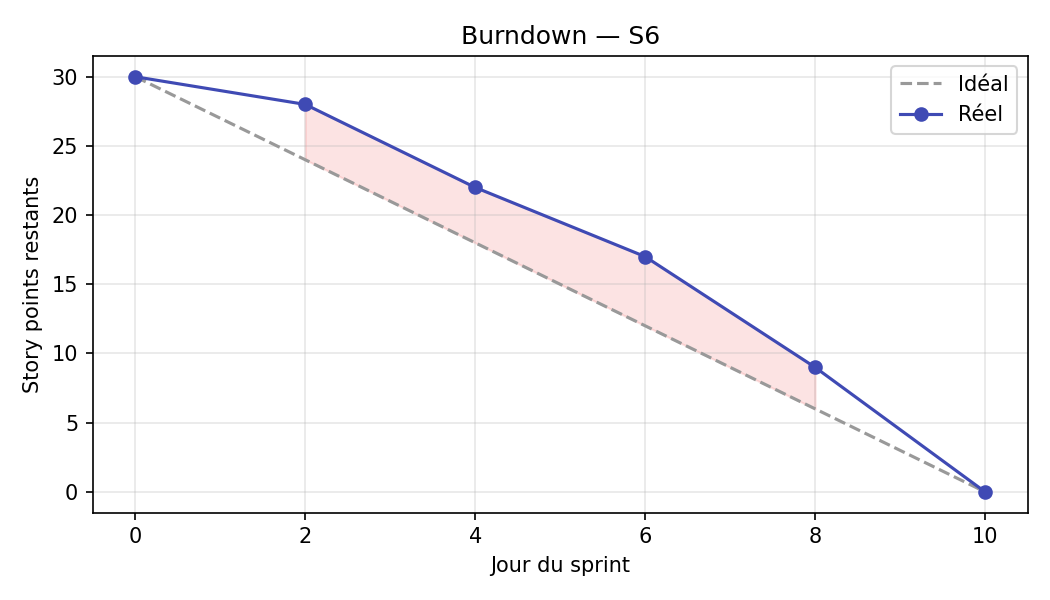
\includegraphics[width=0.85\linewidth]{burndown-s6}
\caption{Burndown du sprint 6 --- Déploiement et démonstration.}\label{fig:burndown-s6}
\end{figure}

\chapter{Extraits de code commentés}
\label{anx:code}

\section{Implémentation de RICE}
\begin{lstlisting}[caption={Scoring RICE normalisé sur [0;100].}]
def score_rice(f: Feature) -> float:
    """RICE = (Reach * Impact * Confidence) / Effort."""
    raw = (f.reach * f.impact * f.confidence) / max(f.effort, 0.1)
    return min(100.0, raw * 1.5)  # normalisation empirique
\end{lstlisting}

\section{Implémentation de WSJF}
\begin{lstlisting}[caption={Scoring WSJF (SAFe).}]
def score_wsjf(f: Feature) -> float:
    """WSJF = Cost of Delay / Job Size."""
    cod = f.business_value + f.time_criticality + f.risk_reduction
    raw = cod / max(f.job_size, 0.1)
    return min(100.0, raw * 4.0)
\end{lstlisting}

\section{Implémentation d'ICE}
\begin{lstlisting}[caption={Scoring ICE.}]
def score_ice(f: Feature) -> float:
    """ICE = Impact * Confidence * Ease, normalise sur [0;100]."""
    raw = f.impact * f.confidence * f.ease
    return min(100.0, raw * 2.5)
\end{lstlisting}

\section{Sprint Planner glouton}
\begin{lstlisting}[caption={Algorithme glouton du Sprint Planner.}]
def plan_sprint(features, velocity, algorithm):
    scored = prioritize(features, algorithm)
    selected, deferred = [], []
    cumulative = 0.0
    for rank, item in enumerate(scored, start=1):
        if cumulative + item.effort <= velocity:
            selected.append({"rank": rank, **item.dict()})
            cumulative += item.effort
        else:
            deferred.append({"rank": rank, **item.dict()})
    utilization = round(100 * cumulative / velocity, 1)
    return {"selected": selected, "deferred": deferred,
            "utilization": utilization, "velocity": velocity}
\end{lstlisting}

\section{Construction de la chaîne RAG (LangChain)}
\begin{lstlisting}[caption={Pipeline RAG avec mémoire conversationnelle.}]
def build_rag_chain(model="gpt-4o", session_id="default"):
    llm         = get_llm(model)
    vectorstore = get_vectorstore()
    retriever   = vectorstore.as_retriever(
        search_type="mmr",
        search_kwargs={"k": 6, "fetch_k": 20},
    )
    memory = ConversationBufferWindowMemory(
        k=10, memory_key="chat_history",
        return_messages=True, output_key="answer",
    )
    return ConversationalRetrievalChain.from_llm(
        llm=llm, retriever=retriever, memory=memory,
        combine_docs_chain_kwargs={"prompt": PO_PROMPT},
        return_source_documents=True,
    )
\end{lstlisting}


\bibliographystyle{plain}
\bibliography{biblio}
\addcontentsline{toc}{chapter}{Bibliographie}

\end{document}
